\documentclass[10pt,a4paper]{article}
\usepackage[utf8]{inputenc}
\usepackage{amsmath}
\usepackage{amsfonts}
\usepackage{amssymb}
\usepackage{graphicx}
\usepackage{enumerate}
\begin{document}

\section{Set Theory}

To demystify mathematics consider
\begin{enumerate}[(i)]
\item What is a theorem?
\item What is a proof?
\end{enumerate}
What if we don't know the answer?

To begin we need
\begin{enumerate}[(a)]
\item an example(s)
\item a nearly related concept
\end{enumerate}


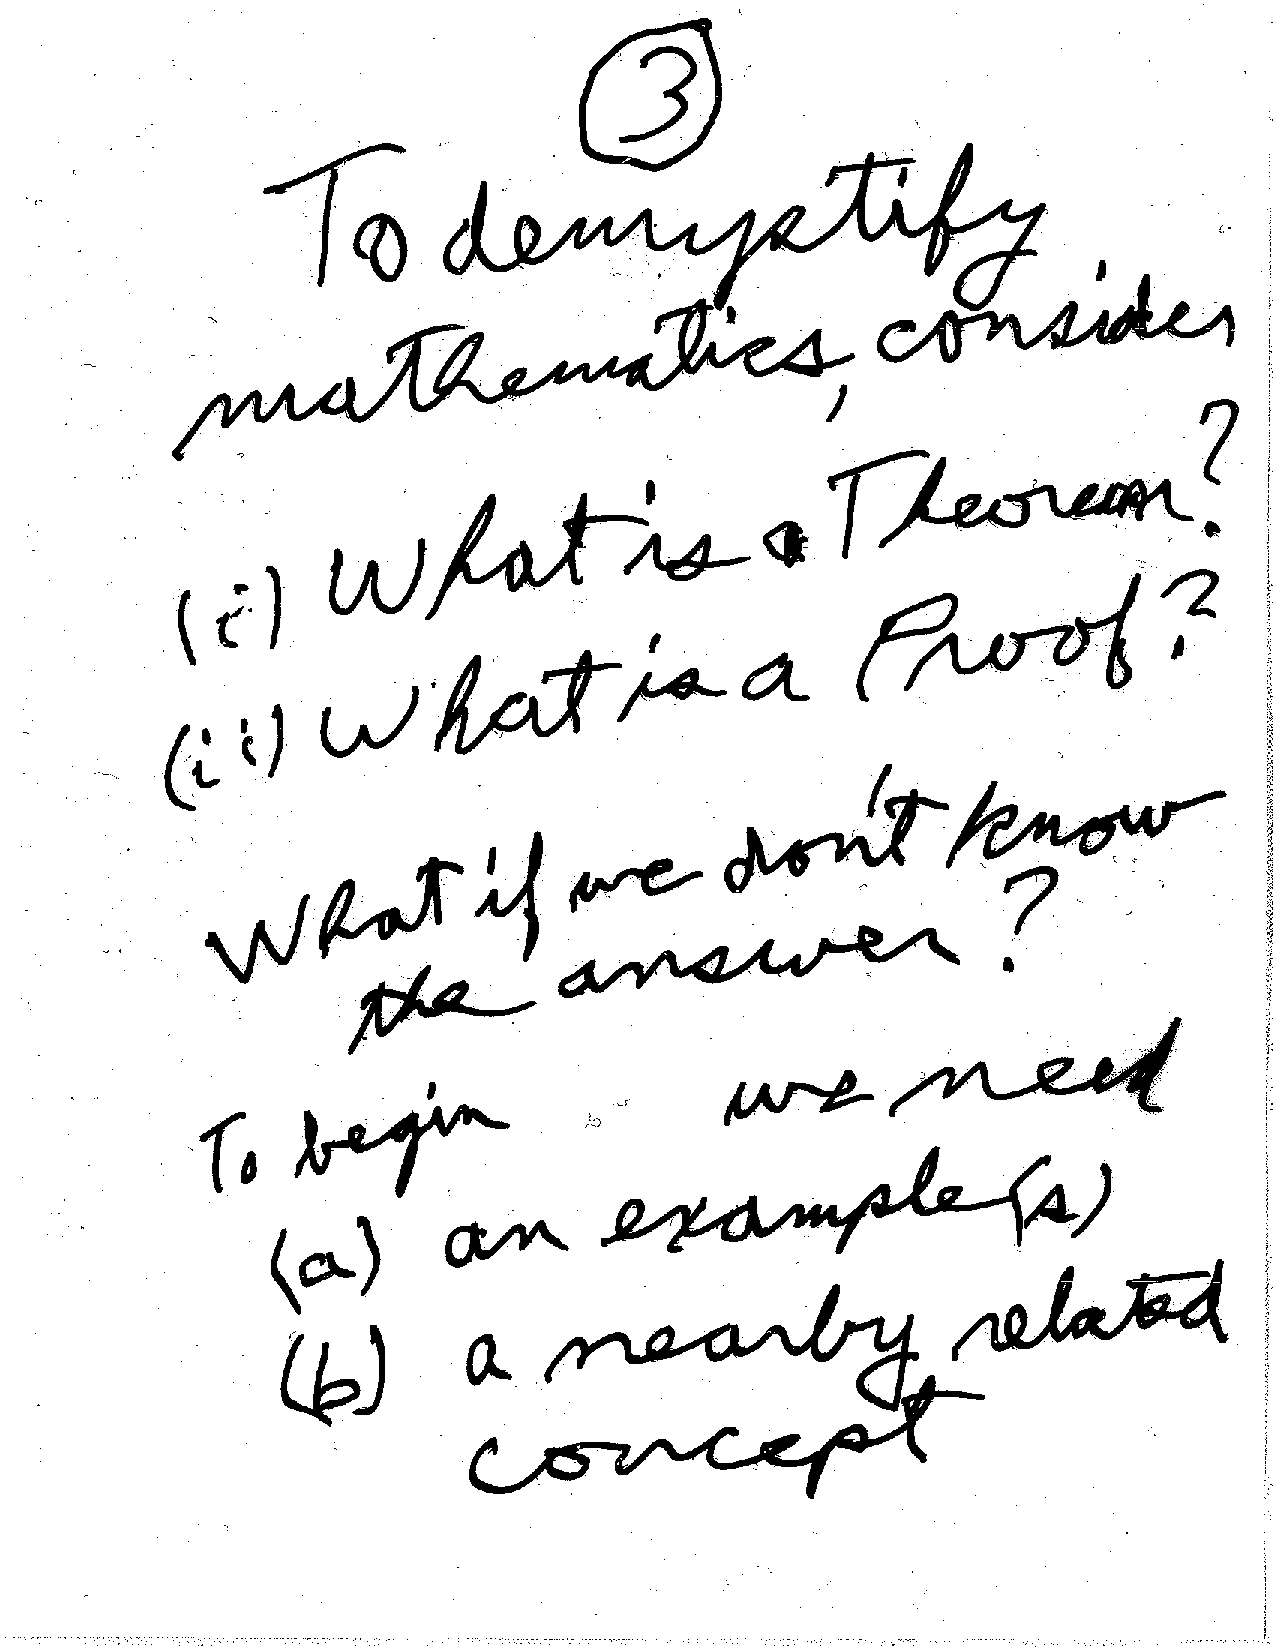
\includegraphics[scale=.5]{Pages/ST_3}

\newpage

Related Concept: Greek Syllogism

\underline{example:}
\begin{enumerate}
\item All men are mortal.
\item Socrates is a man.
\item Therefore, Socrates must die. 
\end{enumerate}

To analyze, recast in set theoretic terms via Venn Diagram.

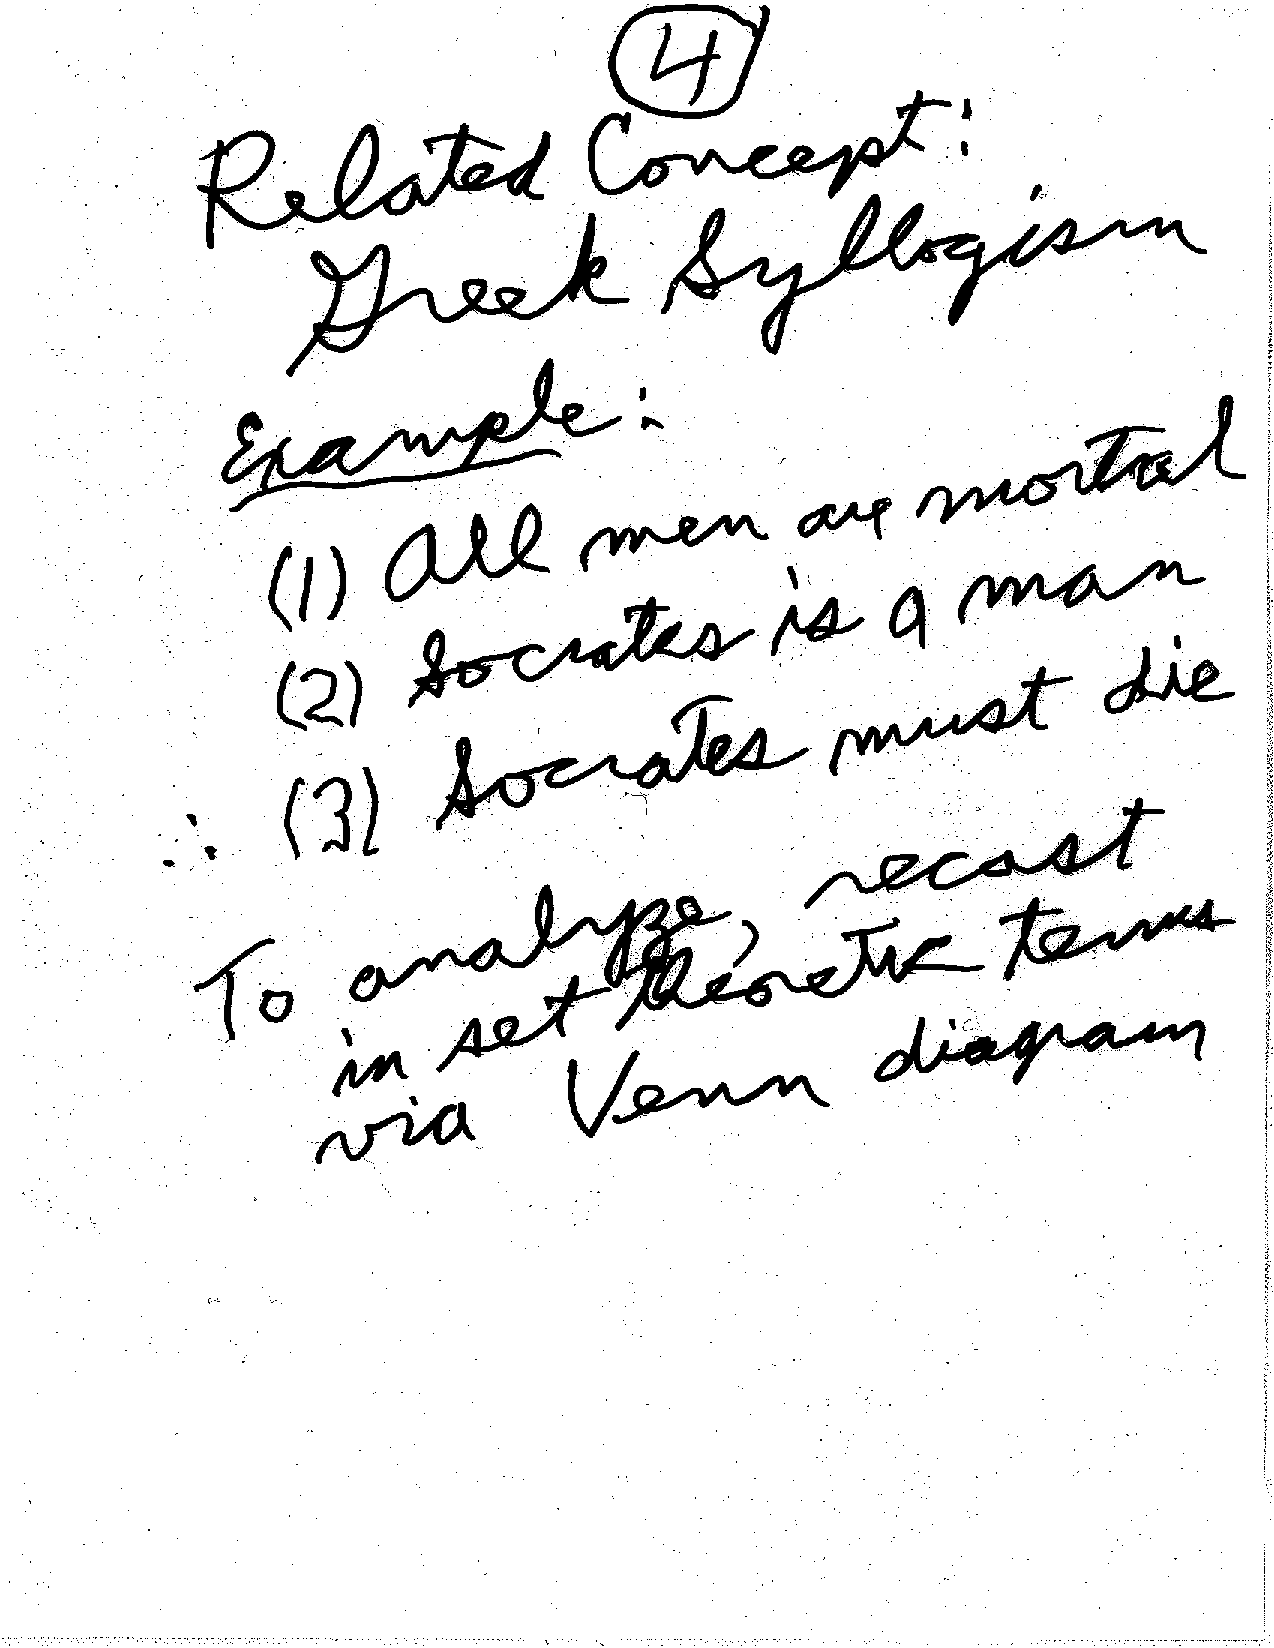
\includegraphics[scale=.5]{Pages/ST_4}

\newpage

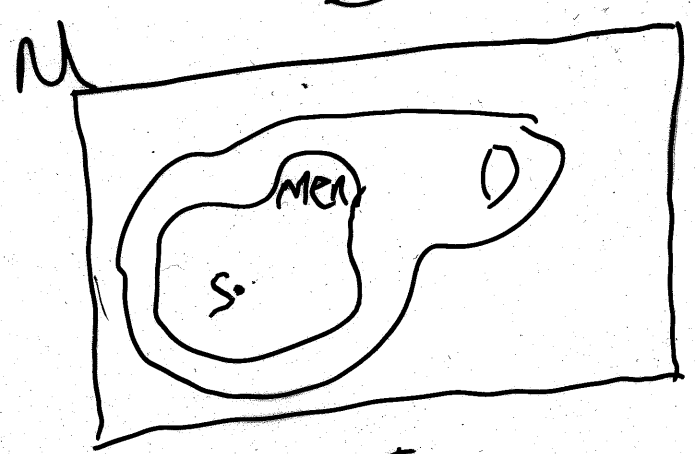
\includegraphics[scale=.2]{Pages/ST_5_im1}

$S$: Socrates\\
$M$: Set of Men\\
$D$: Things that will die\\
$\mathcal{U}$: Things on Earth

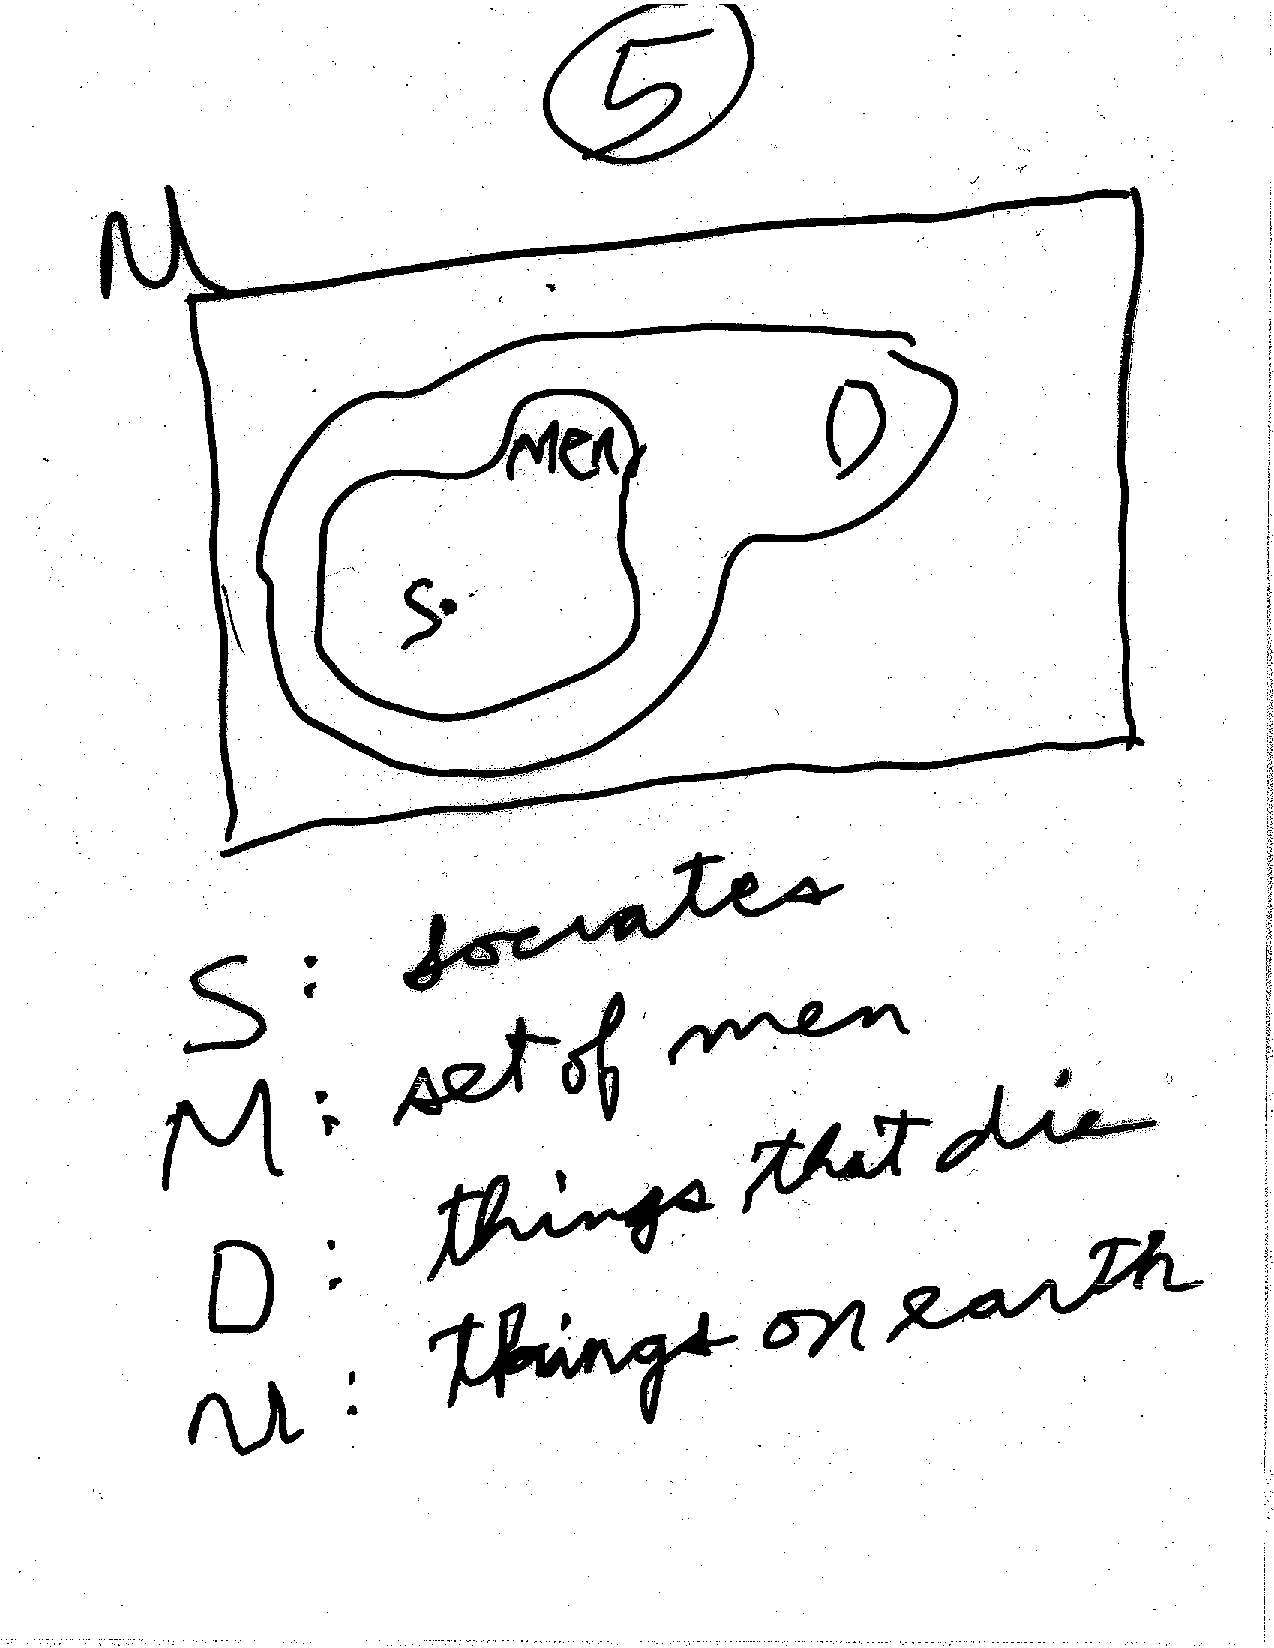
\includegraphics[scale=.5]{Pages/ST_5} 



%Zack: Pages 6,7,8,19,20

%Jack: 21, 9, 10, 11

%Koka: Pages 13, 13A, 22 ,22A, 22B


\section{Generate $\mathbb{N}$}


%Ruth: Pages L4A-L4G




\section{From $\mathbb{Z}$ to $\mathbb{R}$ via ordering}
%Jazz: ZR1-ZR5

%Kyler: ZR6 - ZR10

%Preethika: ZR11-ZR14


\section{Sequence and Limits}

%Aaron: First 2 pages and 48-50
%Hamza: 51-52B

\section{Limit and Convergence}

%Joe: 50-51

%Quinten: 52-53

%Farishta: 53A-54A
Prop let $\{a_n\}$ be a Cauchy sequence in R. Then $\{a_n\}$ is \underline{bdd}.
$P1:\exists N <\infty$ such that for j,k $\geq N \mid a_j - a_k \mid < 1,let$
$B= max \{|a_1|, |a_2|,..., |a_N|\}+1$
for $ 1 \leq j \leq N, |a_j|< B.$
for $ j>N $
$|a_j| = |a_j-a_N+a_N|$
$|a_N| + |a_j-a_N|$
$<|a_N| + 1 \leq B$
Hence $\{a_j\}$ is \underline{bounded}

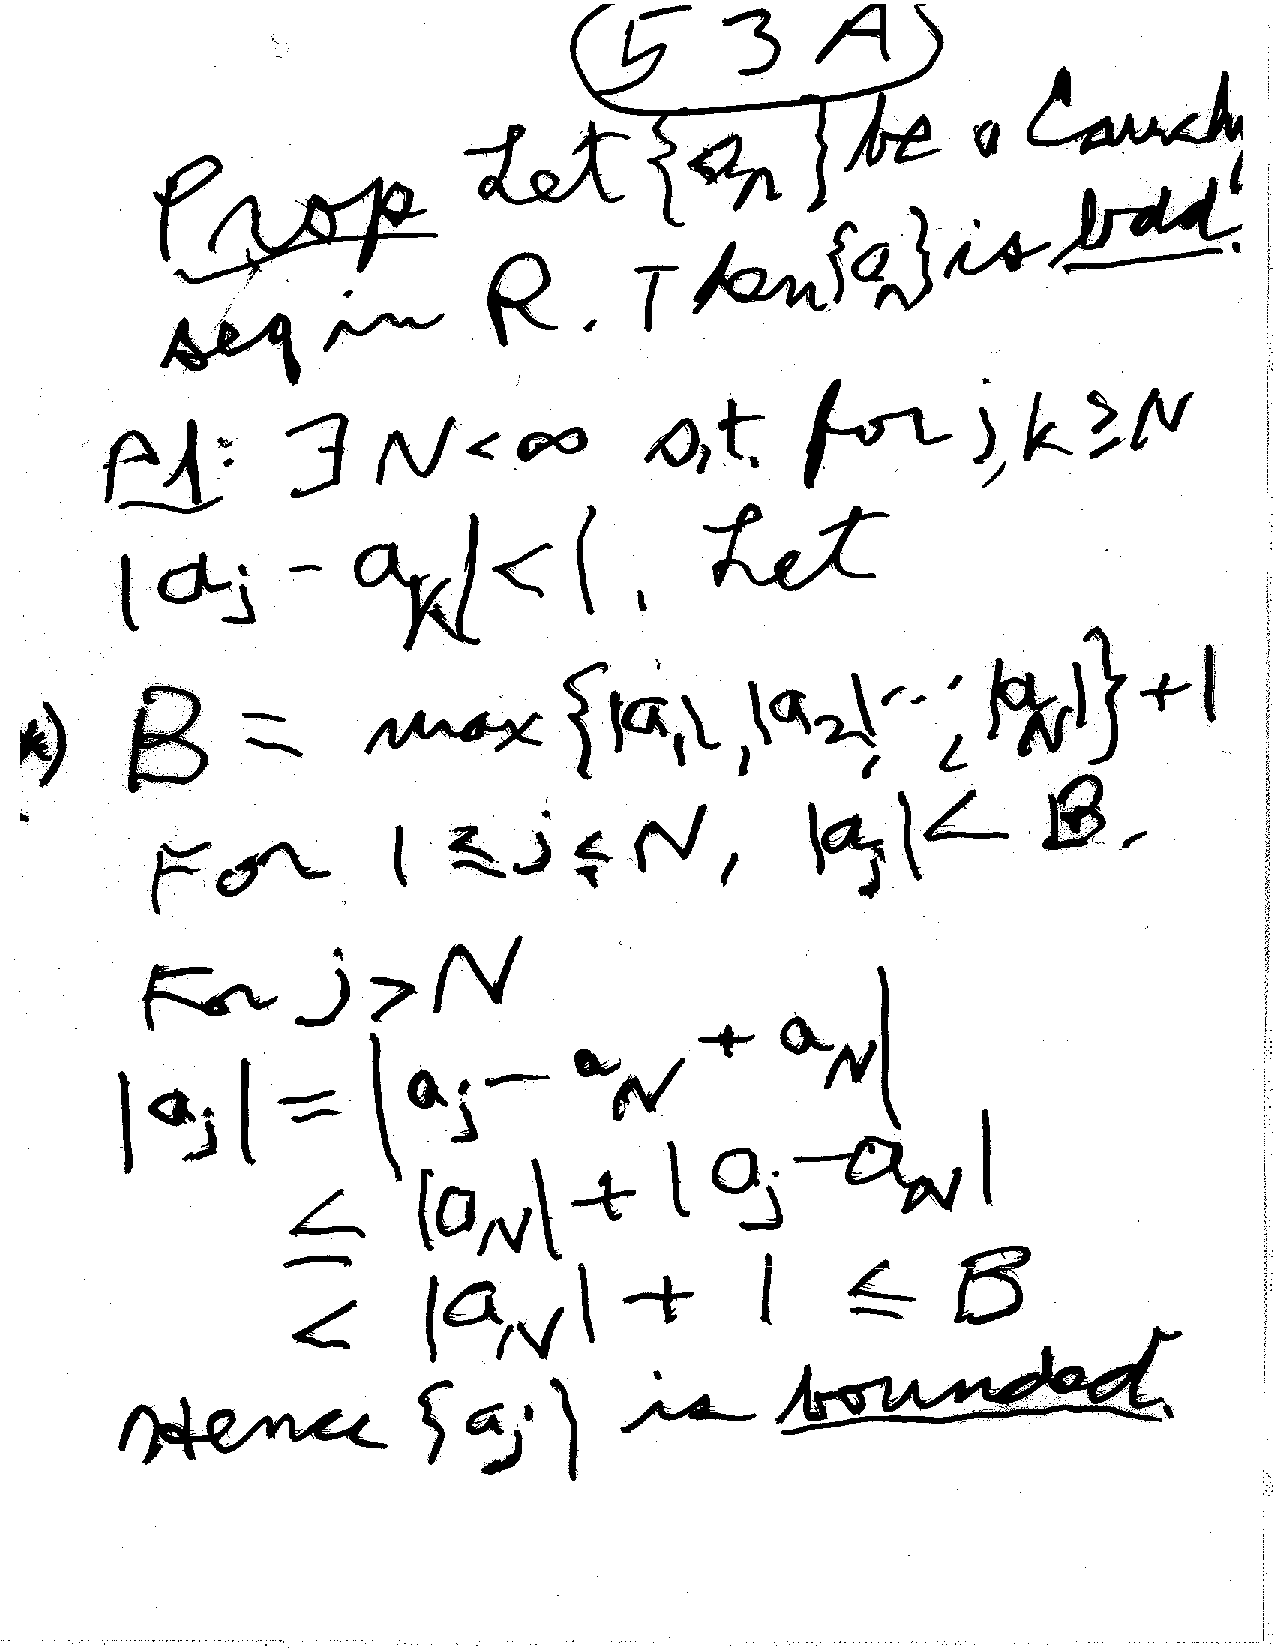
\includegraphics[scale=.5]{Pages/LC_11}

\newpage
\underline{Then} ${a_n}$ con in R if ${a_n}$ is Cauchy
\underline{P1} $| \Rightarrow|$ space $a_n \longrightarrow$ a in R. Take any $\varepsilon > 0. \exists N \varepsilon < \frac {\varepsilon} {2}$ 
$For j,k>, N\varepsilon$ 
$|a_j-a_{k}|=|a_j-a+a-a_k|
\leq |a_j-a|+|a-a_k|
< \frac{\varepsilon}{2} + \frac{\varepsilon}{2}
=\varepsilon$

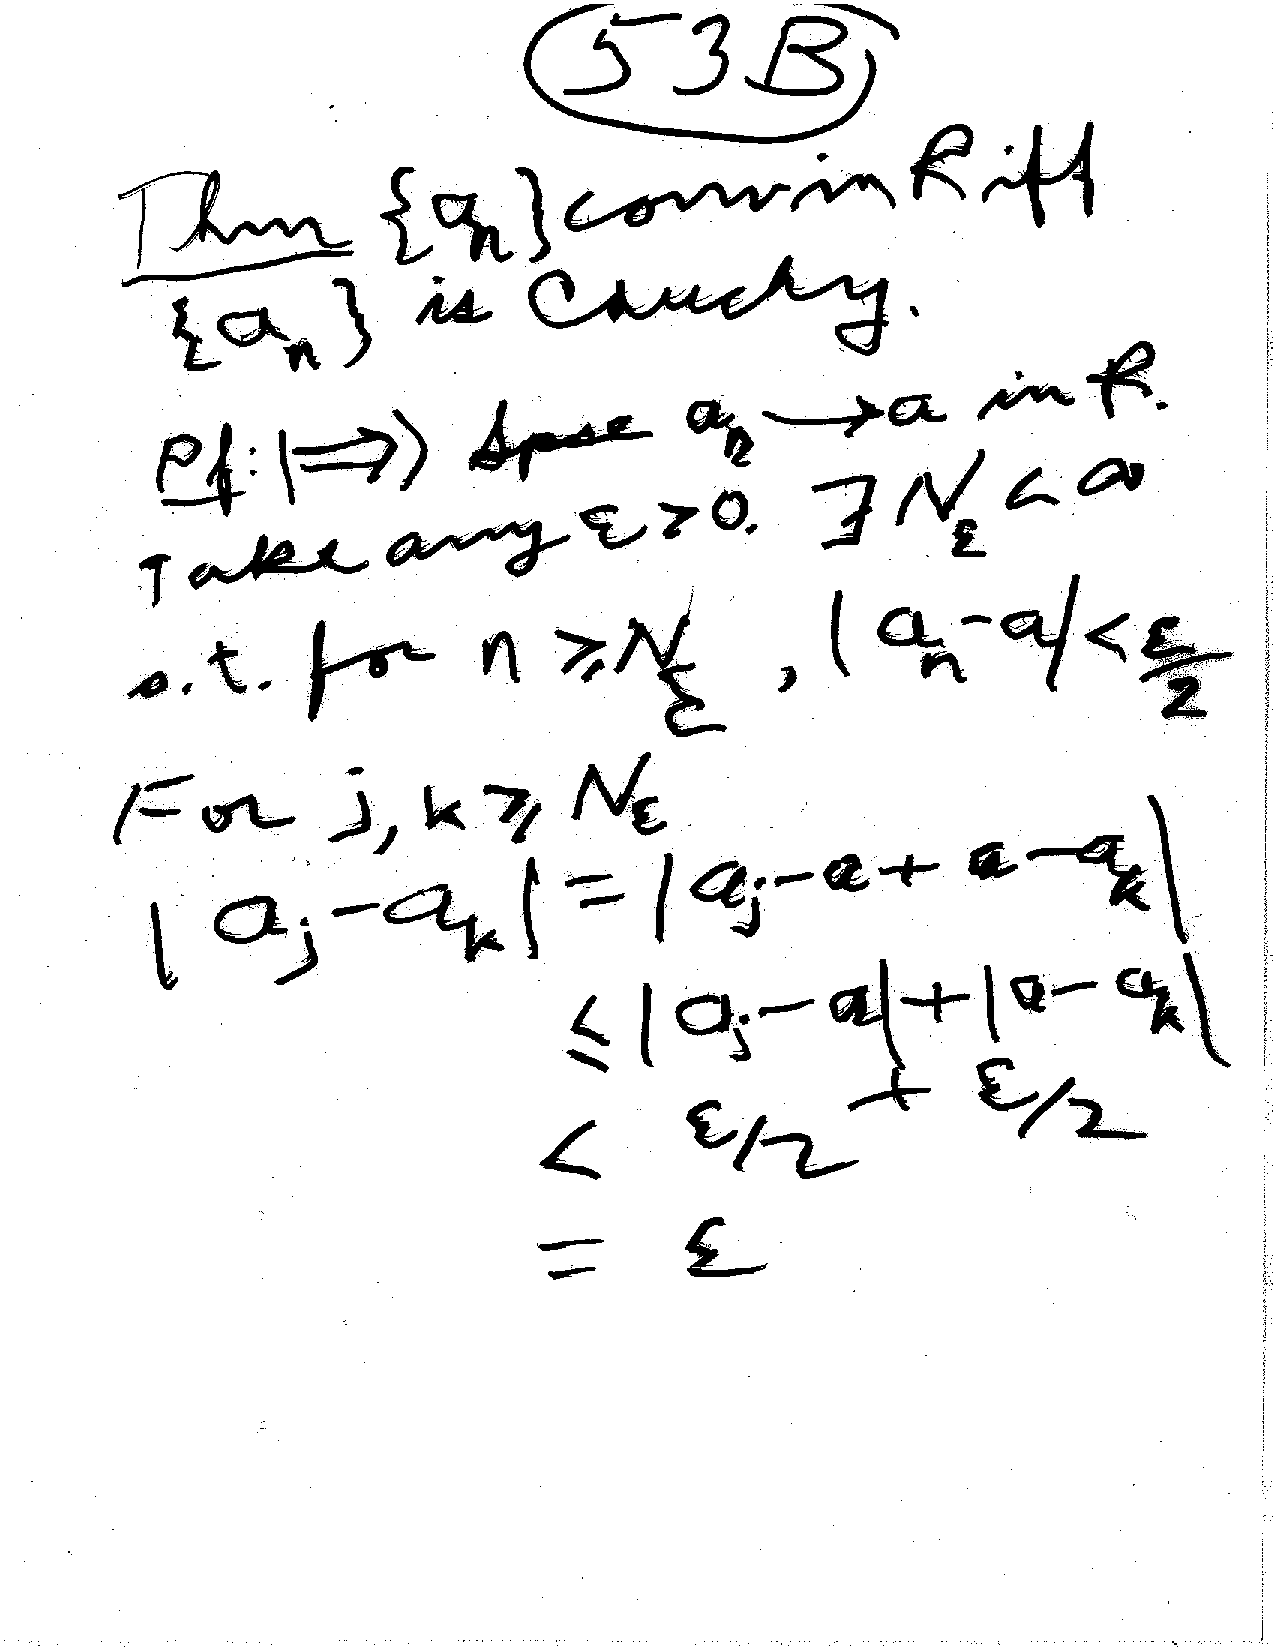
\includegraphics[scale=.5]{Pages/LC_12}

\newpage
$(\Leftarrow)$ space ${a_n}$ is Cauchy.
Then $\exists B < \infty$ such that $|a_n| \leq B$ for all n. more over $\exists 1 \leq n_{1} < n_{2}...$ such as ${a_{n_{k}} :\geq 1}$ is montonic

 w.l.o.g. space $a_{n}, \leq a_{n_2} \leq...$ let $L= rays a_{n_{k}} : k \geq 1$ Then lim $a_{n_{k}}  L (\leq B) k\longrightarrow \infty$ 
Conjecture:$a_j \rightarrow L$

P1: Take away $\varepsilon > O. \exists_\varepsilon < \infty$ s.t. for $k \geq k_\varepsilon |a_{n_{k}} - L| < \frac{\varepsilon}{2}$ for $i,J \geq N_\varepsilon.$ do for $j \geq N_\varepsilon$ and $k \geq N_\varepsilon, |a_j - 4 \leq |a_j - a{n_{k}} - 4$ \\

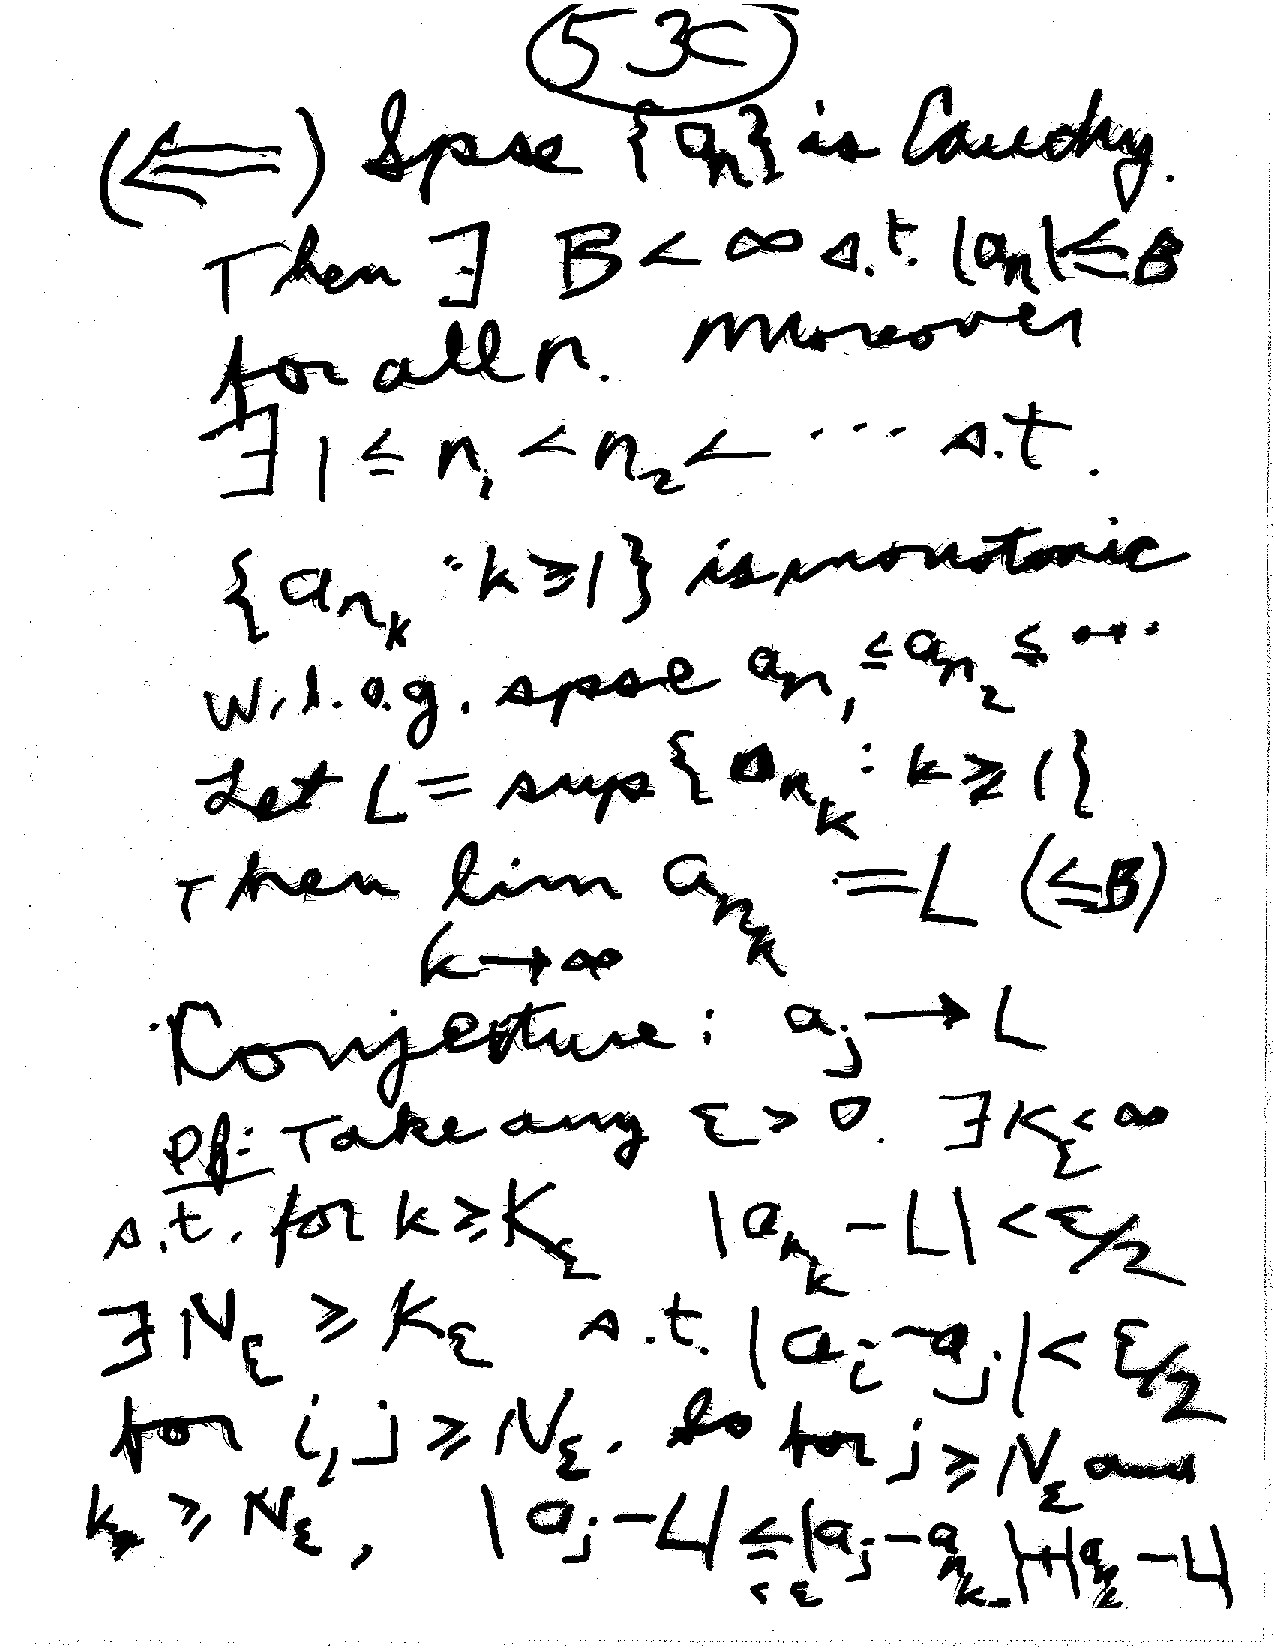
\includegraphics[scale=.5]{Pages/LC_13}



\section{Infinite Series}

%Sukhreet: IS1 - IS 7

%Matthew: IS8 - IS15

%Will: IS16 - IS23

%Rebecca: IS24 - IS32

%Maady: IS33 - IS42

\section{Metric Spaces Part 1}

%Travis: M1 - M5

%Jerome: M6- M10



\section{Metric Spaces Part 2}


%Bryant: M1-M7

%Reshma: M8-M14

%Ethan: M15-M21





\end{document}